\documentclass{article}
\usepackage{amsmath}
\usepackage{parskip}
\usepackage{fullpage}
\usepackage{graphicx}

\title{Deep Learning}
\author{Paolo Bettelini}
\date{}

\graphicspath{ {Resources/} }

\begin{document}

\maketitle
\tableofcontents
\pagebreak

\section{Types of neurons}

\subsection{Brain neurons}

\begin{center}
    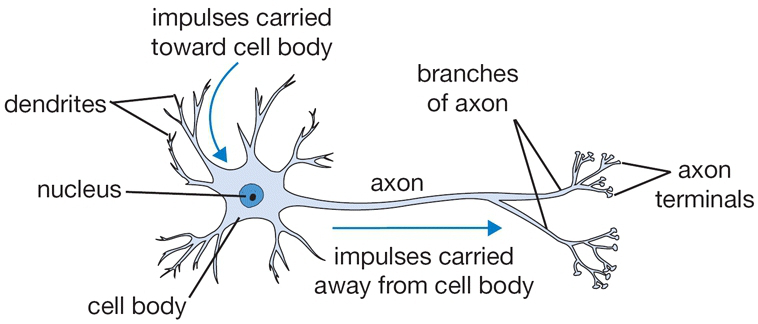
\includegraphics[scale=0.5]{neuron}
\end{center}

\subsection{Linear neurons}

% lecture 1.3

A linear neuron is very simple and computationally limited in what it can do.

\[
    y=b+\sum_{i} x_i w_i
\]

The output \(y\) is given by the bias \(b\) plus the sum of all the input connections \(x_i\) multiplied by their weight \(w_i\).

\subsection{Binary threshold neurons}

Binary threshold neurons output a \(1\) or a \(0\) depending on its weighted value.

Given a threshold \(\theta=-b\)
\begin{align*}    
    z&=b+\sum_{i} x_i w_i \\
    y&=\begin{cases}
        1 \text{ if } z\ge 0 \\
        0 \text{ otherwise}
    \end{cases}
\end{align*}

\subsection{Rectified Linear Neurons or Linear threshold neurons}

They compute a linear weighted sum of their inputs. \\
The output is a non-linear function of the total input.

Given a threshold \(\theta=-b\)
\begin{align*}    
    z&=b+\sum_{i} x_i w_i \\
    y&=\begin{cases}
        z \text{ if } z > 0 \\
        0 \text{ otherwise}
    \end{cases}
\end{align*}

% *picture*

\subsection{Sigmoid neurons}

They give a real-valued output that is a smooth and bounded function of their total input.

The logistic function is often used.

Given a threshold \(\theta=-b\)
\begin{align*}    
    z&=b+\sum_{i} x_i w_i \\
    y&=\frac{1}{1+e^{-z}}
\end{align*}

% *picture*

This function has smooth derivatives that change continuously. \\
This characteristic makes the learning process easier.

\pagebreak

% lecture 1.5

\section{Types of learning}

\subsection{Supervised learning}
Each training consists of making the network guess the target output \(t\) for a certian input \(x\), given the difference between the correct target and the guess we tweak the network.

There are two type of supervised learning

\subsubsection{Regression}
The target output is a numeric value of a vector of values. 
[\ldots]

\subsubsection{Classification}
The target output is a class or label. Usually either \(1\) or \(0\).
There could also be multiple labels.
[\ldots]

\subsection{Reinforcement learning}
\subsection{Unsupervised learning}



\end{document}